\documentclass{standalone}
\usepackage{tikz}
\usetikzlibrary{arrows,shapes,shadows,positioning}

\tikzset{
  %Define standard arrow tip
    >=stealth',
  %define style for boxes
  punkt/.style={
    rectangle,
    rounded corners,
    draw=black,very thick,
    text width=7.5em,
    minimum height = 2em,
    text centered},
  punkp/.style={
    rectangle,
    dashed,
    rounded corners,
    draw=black,very thick,
    text width=7.5em,
    text centered, 
    anchor=north,
    minimum height = 2em},
  %define style for arrows
  myarrow/.style={
    ->, 
    >=open triangle 90, 
    shorten >=1pt, 
    thick}
}


\begin{document}

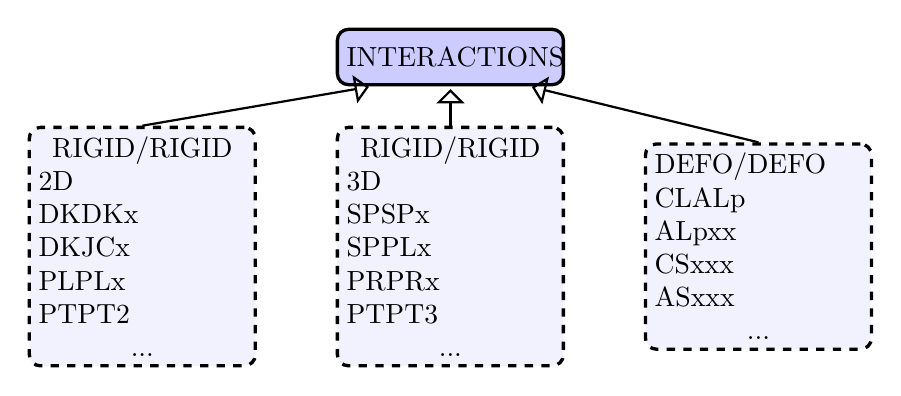
\begin{tikzpicture}[node distance=1cm, auto,]
%nodes
\node[punkt, fill=blue!20] (interactions) {INTERACTIONS};

\node[punkp, below = 0.5cm of interactions,fill=blue!5] (CT3D) 
     {RIGID/RIGID 3D 
      \newline SPSPx \newline SPPLx \newline PRPRx \newline PTPT3 \newline ...};
\node[punkp, below = 0.5cm of interactions, left=of CT3D, fill=blue!5] (CT2D) 
     {RIGID/RIGID 2D
      \newline DKDKx \newline DKJCx \newline PLPLx \newline PTPT2 \newline ...};
\node[punkp, below = 0.5cm of interactions, right=of CT3D, fill=blue!5] (DEFO) 
     {DEFO/DEFO \newline CLALp \newline ALpxx \newline CSxxx \newline ASxxx \newline ...};

\draw[myarrow] (CT2D.north) -- ([xshift=-1cm]interactions.south);
\draw[myarrow] (DEFO.north) -- ([xshift= 1cm]interactions.south);
\draw[myarrow] (CT3D.north) -- (interactions.south);

\end{tikzpicture}

\end{document}
